`\chapter{Models}
With this chapter we explore some of the most common forecasting models for traffic datasets.  These models are meant to be used as a baseline from which to compare our results.  Also, in chapter 4 the models presented here are incorporated into an ensemble forecasting model.  The models selected for this work are:

\begin{itemize}
	\item Seasonal auto regressive integrated moving average
	\item Historic average
	\item Time delayed neural network
	\item Support vector regression
\end{itemize}


Also in this chapter, we introduce the metrics which will be used for our analysis.  We feel this analysis useful to empirically demonstrate the various forecasting capabilities of these established models.

Some of the discussions of models within this chapter make mention of our datasets.  These datasets are described in detail in Chapter 3.  We chose to describe the specifics of our forecasting models prior to our datasources because we believe this makes for a more coherent paper.

\subsection{Notation}
As already stated, we define a time series dataset used within as  $\{x_{t}^{(m)}\}$.  Each $x_{t}^{m}$ is an aggregate of the readings from sensor $m$ reading at time block $t$.  In total the number of time blocks are represented by $N$.

Forecasts for a given model $k$ from the set of all models $K$ are represented by 
\begin{equation}
y_{t + 1}^{k, m} = f(x_{t}, ..., x_{1}; \theta_{k}).
\end{equation}
\noindent
Thus the forecast of $x_{t + 1}$ is a function of all past data and some trained parameterization $\theta_{k}$ for that model.  For this work we forecast a model for each individual sensor and for convenience often drop the $m$ and $k$ from our forecast notation.  Also, in this work we need to forecast more than one time step into the future.  Future forecasts are performed through iterative one step ahead forecasts.    An example of a forecast two time steps ahead of current time $t$ is given by 
\begin{equation}
y_{t + 2} = f(y_{t + 1}, x_{t}, ..., x_{1}; \theta_{k}).
\end{equation}
\noindent
Such a forecast is simply the forecast for one time step into the future but now with the forecasted value of $y_{t + 1}$ used as the most recent datapoint to forecast $y_{t + 2}$.  Forecasting in this nature allows for forecasts any number of time steps into the future.

Another useful time series used in this work is the residual dataset defined as
\begin{equation}
r_{t,\delta} =  x_{t + \delta} - y_{t + \delta}.
\end{equation}
This set of residuals is the difference between the raw data and a forecasting function operating $\delta$ time steps into the future. 


\subsection{Forecast Error Measurements}
There are a multitude of various forecasting error measurements that have been used to assess forecast accuracy.  Expert recommendation of which forecast error measurement to use for what types of data has changed over time.  Armstrong \cite{Armstrong2001, Yokuma1995} found that root mean squared error (RMSE) was by far the most popular error measurement in 1981 among academics.  However, by 1995 RMSE preference by academics had dropped by roughly half and mean absolute percentage error (MAPE) was the preferred error measurement. 

For this work, to coincide with expert opinion on forecast error measurements, we use both mean absolute scale error (MASE) \cite{Hyndman2006, Hyndman2006a} and RMSE as cost functions to compare our forecasting accuracy.  RMSE was selected due to its simplicity and ubiquity within the forecasting community.  MASE was selected for it being both a modern derivation of MAPE and for its accuracy in places where MAPE does not provide adequate results.  

Also, because much of the focus of our work is interested in reducing inaccurate forecasts during the presence of some anomalous event, we introduce another forecasting measurement which we call root mean squared error outside of noise against naive (RMSEONAN).  This metric provides a convenient way to measure the improvement our approach yields which is not easily captured by RMSE and MASE.

\bigskip
\noindent \textbf{RMSE} \\
One of the most common error functions used to determine the quality of a set of forecasts.  It measures the average difference between two time series.  Due to its squared error term, this measurement is not a good indicator of error between distinctly different datasets.  For our work comparing the input series $x$ and the forecast series $y$ RMSE performs adequately.
\begin{equation}
RMSE_{\delta} = \sqrt{\frac{\sum_{t = 1}^{N - \delta}{(x_{t + \delta} - y_{t + \delta})^{2}}}{N - \delta}}
\end{equation}

\bigskip
\noindent \textbf{MASE} \\
Mean absolute scaled error was developed to be a generally applicable measurement of forecast error.  The metric is especially useful for datasets with intermittent demand unlike the commonly used MAPE score.  The reason it works well with intermittent time is that it will not return undefined or infinite values unless the compared datasets are equal \cite{Hyndman2008}.

\begin{equation}
MASE_{\delta} = \frac{\sum_{t = 1}^{N - \delta}{r_{t, \delta}}}{\frac{N}{N - 1}\sum_{i = 2}^{N}|y_{i} - y_{i - 1}|}
\end{equation}

\bigskip
\noindent \textbf{RMSEONAN} \\
Root mean squared error outside noise against naive measures a forecast's accuracy during its worst case scenarios.  This is performed by measuring the sum of squared errors of forecasts outside a prescribed boundary.  We compute this boundary from the forecasting accuracy of a naive forecaster.  For our work, we consider the naive forecaster to be the historical average of the data for a given time.  

Most of the results of this work deal with boundaries set by one standard deviation of the residual dataset formed but the historic average (naive) model.  RMSEONAN is defined as

\begin{equation}
RMSEONAN_{\delta, \sigma} = \frac{\sqrt{\sum_{t = 1}^{N - \delta}{A(r_{t, \delta}; \sigma)^{2}}}} {N - \delta}.
\end{equation}

Where $A(r_{\delta}; \sigma)$ is 

\begin{equation}
A(r_{t, \delta}; \sigma_{t}) = \begin{cases}
			r_{t, \delta}    &    \text{If }r_{t, \delta} \ge \sigma_{t} \\
			0                     &    \text{otherwise.}
			\end{cases}
\end{equation}

$\sigma_{t}$ is the standard deviation of the data at that time step for that given day.  For certain comparisons, it is useful to use $n*\sigma$ with values of $n > 1$.  

Notice that this function is an average of all values of $A(r_{\delta})$.  This is because RMSEONAN is used to compare between multiple forecasting algorithms of the same dataset the total effect of sufficiently inaccurate forecasts (by sufficiently inaccurate, we mean any forecast outside a defined  accuracy boundary).  If we were to measure only values where $A(r_{\delta}) > 0$, then an average value is not able to distinguish between forecasting models that leave few sufficiently inaccurate forecasts and many inaccurate forecasts assuming they are of similar value.  

An example demonstrating the regions summed by RMSEONAN is given by ~\ref{fig:dem_RMSEONAN}.  In this image, only the area of the green spaces are squared and summed towards RMSEONAN.  All other regions are zero.  The large salmon colored region is the area that is one standard deviation for all days at that time for the residual dataset.

\begin{figure}[t]
	\begin{center}
		\includegraphics[width = .8\linewidth]{demonstration_RMSEONAN}
	\end{center}
	\caption{Demonstration of the area measured by RMSEONAN.  Only the solid green regions are measured.  These regions correspond with forecasting errors outside a prescribed boundary which in this case is one standard deviation from the mean for that given period of time.}
	\label{fig:dem_RMSEONAN}
\end{figure}

%MODELS
\subsection{Seasonal ARIMA model}
The Auto Regressive Moving Average Model (ARMA) or derivations on its form (Auto Regressive Integrated Moving Average, Seasonal Auto Regressive Moving Average, $etc$) have been used in numerous forecasting applications from economics to vehicle traffic systems.  While we have been unable to find ARMA based models used on building occupancy data directly, we have found it used to forecast building energy usage and vehicle occupancy \cite{Williams2003, Hong2011, Newsham2010, Howard2013, Fernandez2011}.  Due to ARIMA models having a strong forecasting accuracy and frequent academic use, we believe it serves as an excellent baseline of comparison for a forecasting problem.  

Our building and traffic data has periodic trends and a non stationary mean, thus from the class of ARIMA models, we believe a seasonal ARIMA model is best suited to fit our data.  The seasonal ARIMA model is defined as:
\begin{equation}
\label{eq:sarima}
\phi_{p}(B)\Phi_{p}(B^{s})\nabla^{d}\nabla^{D}_{s}T_{t} = \theta_{q}(B)\Theta_{Q}(B^{s})e_{t}
\end{equation}
\noindent
where $\{T_{t}\}$ is our observed time series and $\{e_t\}$ represents an unobserved white noise series ($e_{t} \sim N(0, \sigma^{2})$) the values of which are computed through model training and are not known a priori.  $B$ is the backshift operator which is a function that allows access to older time readings.  For example $BT_{t} = T_{t-1}$ and $B^{5}T_{t} = T_{t-5}$.  $\nabla^{D}_{s}$ is the seasonal difference operator ($\nabla^{D}_{s}T_{t} = (1 - B^{s})^{D}T_{t}$) and $\phi,\  \Phi,\  \theta,\ \Theta$ are trainable parameters.  

Seasonal ARIMA models are notated as
\begin{equation}
ARIMA(p,d,q)(P,D,Q)_{s}
\end{equation}
where $p$ is the number of autoregressive terms, $d$ is the number of differences and $q$ is the number of moving average terms.  $P$, $D$, and $Q$ all correspond to the seasonal equivalents of $p$, $d$, and $q$.  The parameter $s$ is the seasonality of the model.  For a full discussion of seasonal ARIMA models see Box and Jenkins \cite{Box2008}.

Forecasting from this model is performed by iteratively forward feeding values of the model into itself.  Since the set of residuals $e$ from a properly trained seasonal ARIMA model is described by a white noise Gaussian distribution $N(0, \sigma^{2})$, we can take the expected value of the residual at time $e_{t + 1}$ to be 0.  This leaves us with the following forecasting equation: 
\begin{equation}
\label{eq:sarima}
\phi_{p}(B)\Phi_{p}(B^{s})\nabla^{d}\nabla^{D}_{s}T_{t + 1} = \theta_{q - 1}(B)\Theta_{Q - 1}(B^{s})e_{t}
\end{equation}


\subsubsection{Fitting a Seasonal ARIMA}

Finding the correct values of $p, d, q, P, D, Q, s$ is traditionally a hard problem.  To fit our parameters we use a method similar to Williams \cite{Williams2003}.  The underlying math of ARMA models stems from a linear filter operating on input from a stationary stochastic process.  ARIMA models were created to handle non-stationary data by differencing the data to induce stationarity.  A necessary step in fitting a ARIMA model to the data is first to determine the steps necessary to make the time series weakly stationary.  For a time series to be weakly stationary two conditions must be satisfied: The expected value of $x^{(t)}$ is the same for all $t$ and the covariance between any two observations depends only on the lag.  

\begin{table}[t]
\centering
\caption{The parameter values that were fit for MERL and CSMBB datasets for a Seasonal ARIMA model}
\begin{tabular}{|c|c|c|c|c|c|c|c|} \hline
Dataset & $p$ & $d$ & $q$ & $P$ & $D$ & $Q$ & $s$\\ \hline
MERL & 0 & 0 & 1 & 0 & 1 & 5 & 78\\ \hline
CSMBB & 0 & 1 & 1 & 0 & 1 & 3 & 72\\ \hline
DENVER & 1 & 0 & 1 & 0 & 1 & 1 & 168\\ \hline
\end{tabular}
\label{fig:sarimatab}
\end{table}

As a verification of our model, we applied the LJung-Box test \cite{Ljung1978} on our set of residual data for each model.  This tests if any of the auto correlation values on the residual dataset are significantly different from 0.  To be valid, the LJung-Box test should return a value of $p > 0.05$.  All of our residual sets passed: $p = 0.9964$ for MERL and $p = 0.1072$ for CSMBB and $p = 0.1266$ for Denver.  Our final model parameters can be seen in ~\ref{fig:sarimatab}.  Notice that the season is different for each model due to a difference in window of time for each day that we extracted data.

\begin{figure}[]
	\begin{center}
		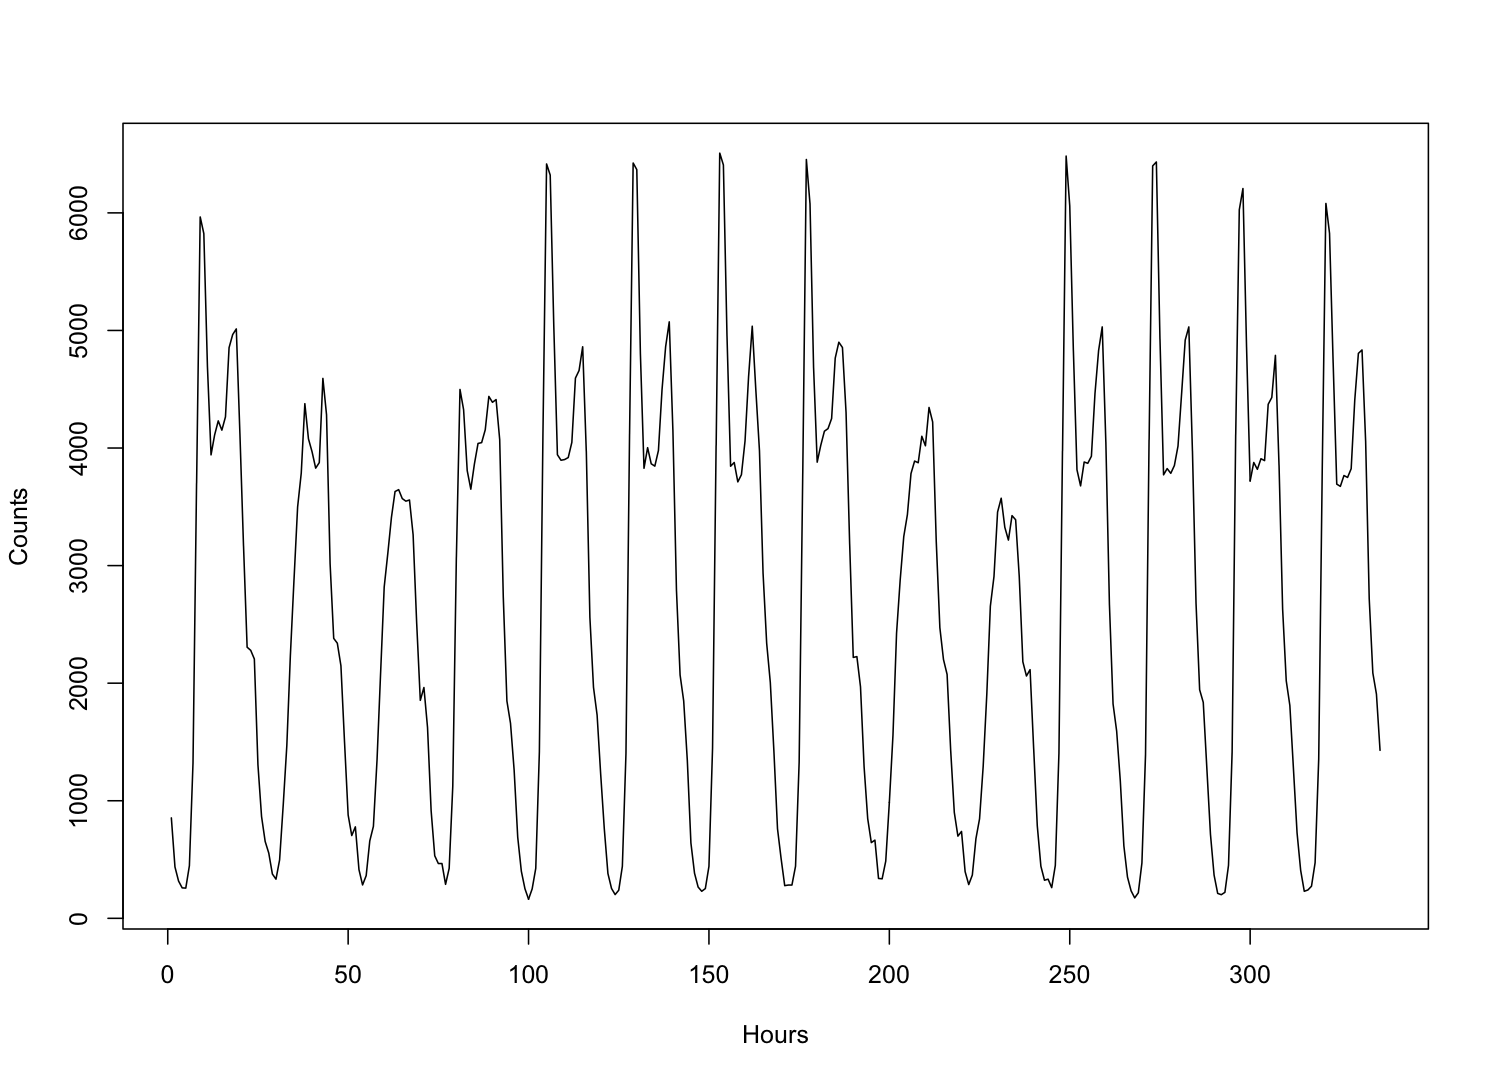
\includegraphics[width = .6\linewidth]{denver_counts.png}
	\end{center}
	\caption{Raw counts of Denver data for one sensor over a two week period.}
	\label{fig:denver_raw_data}
\end{figure}

In general it is difficult to prove stationarity, but there exists a number of methods which assist in determining if a time series is close enough to stationary to be modeled by an ARMA model.  Visual inspection of both the raw data and the autocorrelation function is a useful tool to test for stationarity.  ~\ref{fig:denver_raw_data} shows the raw counts values at hourly lags of vehicle counts for one sensor over a two week period from the Denver dataset.  The data shows no constant mean and thus can not be stationary.  The graph of autocorrelation values shows local peaks every 24 hours with a significant peak at one week of lag (168 hours).

Intuitively a one week seasonal difference should yield a stationary time series and visually, outside of an anomalous reading, Figure~\ref{fig:lag_data} shows such stationarity.  Applying the Kwiatkowski-Phillips-Schmidt-Shin (KPSS) \cite{Kwiatkowski1992} test for stationarity on the seasonally differenced data confirms the visual inspection.  Using R's implementation of KPSS gives a p-value greater than 0.1.  This is significantly higher than the standard value to reject the stationarity hypothesis of 0.05.  

\begin{figure}[t]
\begin{center}
\subfloat[][Seasonal difference counts] {
\includegraphics[width=0.45\textwidth]{lag_counts.png}
%\label{fig:acf_counts}
}
\subfloat[][Autocorrelation of seasonal difference counts] {
\includegraphics[width=0.45\textwidth]{acf_lag.png}
%\label{fig:acf_lag}
}
\end{center}
\caption{One week seasonal difference counts and autocorrelation over a two week period.}
\label{fig:lag_data}
\end{figure}

Most of the input parameter values for seasonal ARIMA models tend to be 0, 1, 2, or 3 \cite{Box2008}.  Due to this small range of input values the total input space is relatively small (Six parameters with four possible values equates to $4^6 = 4096$) allowing us to apply a brute-force search for the best model.  Model performance is determined by the Akaike information criterion (AIC) \cite{Akaike1974}.  Our optimal model is a seasonal ARIMA $(1,0,1)(0,1,1)_{168}$.  

\begin{figure}[h]
\begin{center}
\includegraphics[width=0.8\textwidth]{broncos_predicted.png}
\end{center}
\caption{One-step ahead prediction for a sample week.  Black line is original data.  Red line is forecasted data.  Dotted box shows an example of mis-forecasting due to a broncos game.}
\label{fig:arima_prediction}
\end{figure}

Verifying our seasonal ARIMA fit is accurate ~\ref{fig:arima_prediction} shows an example of one-step ahead prediction performed on a sample week of test data.  The mean absolute percentage error (MAPE) for this week was approximately 8.2\%.  This MAPE is close to the results from other authors on other vehicle traffic datasets \cite{Williams2003,Smith1997}.  Also, for \ref{fig:arima_prediction} the dotted line boxes a time when a Broncos game was occurring.  Forecasting during the Broncos game was initially low while traffic was unusually high as people were traveling to the game and then too high for much of the duration of the game.  We discuss our approach to solving such misforecasts in Chapter 5.


\subsection{Historic average}
This model is simply the per day average of readings at each time step.  For certain types of data this model is has been shown to be more accurate than seasonal ARIMA forecasting \cite{Newsham2010}, specifically when the data has a strong historic correlation.  Average forecasts have the advantage of being extremely computationally fast and having a forecast accuracy that does not depend on the forecasting horizon.  This result will be shown later.


\subsection{Time delayed neural networks}

Time delayed neural networks (TDNN) are a special subset of regression neural networks where the input data is a local history of data from the time series.  This special class of neural networks have been used frequently traffic forecasting literature \cite{Abdulhai1999, Ishak2003}.  Commonly the output is a single point forecast from that same time series at some point $t + \delta$ in the future.   The form of our 1 hidden layer time delayed neural network is:
\begin{equation}
y_{t + 1} = \phi \{ \sum_{j = 1}^{J} w_{j}\psi_{j} \bigg[ \sum_{l = 0}^{m}w_{ji}x_{t - l\delta} + w_{j0} \bigg] + w_0 \}
\end{equation}
\noindent where $\phi\{\bullet\}$ is a linear activation function on the output layer and $\psi[\bullet]$ is the standard sigmoid function.  A visual representation of the node architecture of a time delayed neural network is displayed in ~\ref{fig:tdnnarch}.

\begin{figure}[h]
	\centering
		\includegraphics[width = .8\linewidth]{time_delay_neural_network.png}
		\caption{Architecture of a time delayed neural network with $m + 1$ inputs and J outputs \cite{Hansen2003}.}
	\label{fig:tdnnarch}
\end{figure}

Forecasting is performed by computing the output for a $m + 1$ length window of time and then iteratively forecasting a set of time steps in the future by using forecast data as inputs into the next forecast. 

The number of input nodes and hidden nodes for each dataset is given in ~\ref{fig:tdnntab}.

\begin{table}[h]
\centering
\caption{Number of delayed input nodes and hidden nodes for MERL and CSMBB datasets}
\begin{tabular}{|c|c|c|} \hline
Dataset & Delayed input nodes & Hidden nodes\\ \hline
MERL & 15 & 8\\ \hline
CSMBB & 12 & 8\\ \hline
DENVER & 6 & 6\\ \hline
\end{tabular}
\label{fig:tdnntab}
\end{table}


\subsection{Support Vector Regression}
Support vector regression (SVR) is a universal learning method which offers a powerful way to forecast time series.  It has been used in the past successfully to forecast travel times and vehicle counts for roadway traffic systems \cite{Wu2004, Wei2013, Wei2012, Howard2013}.  Many of these empirical studies have demonstrated SVR as outperforming other forecasting techniques including ARIMA and TDNN.

The support vector machines was developed by Vapnik \cite{Vapnik1998}.  SVM's use structural risk minimization to find an minimal upper bound on some expected risk.  As training support vector machines to be used for regression is not done in the same way as other time series models, we first had to transform our dataset to a series of examples with a fixed window.  For a fixed window of size $w$, training input data is of the form $\{x_{t}, x_{t - 1}, ..., x_{t - w + 1}\}$.  Target data is of the form $x_{t + 1}$.  Thus the training examples which we provided to our SVM was $\{x_{t + 1}, [x_{t}, x_{t - 1}, ..., x_{t - w + 1}]\}$.

The general formulation for support vector regression is to minimize the following:

\begin{equation}
	\begin{split}
	\min \frac{1}{2}\|w\|^{2} + c \sum_{i = 1}^{n}(\epsilon_{i} + \epsilon^{*}_{i}) \\
	\begin{cases}
		y_{i} - f(x_{i}, w) \le \gamma + \epsilon^{*}_{i} \\
		f(x_{i}, w) - y_{i} \le \gamma + \epsilon_{i} \\
		\epsilon_{i}, \epsilon_{i}^{*} \ge 0, i = 1, \ldots, n
	\end{cases}
	\end{split}
\end{equation}

From this formulation the function $f()$ is the regression function, $w$ are the parameters of the regression function $f()$, $\gamma$ is loss function sensitivity and finally $\epsilon$ are the slack variables which measure the deviation of training samples.  

To perform SVR training we used the popular $libsvm$ package.  Because parameter selection is a notoriously difficult problem for SVR, we followed the guidelines as outlined by Hsu, Chih-Chang and Lin, creators of the libsvm package \cite{Hsu2003}.  We first scaled the data by normalizing it between $[0, 1]$.  Then we searched for our best values of $C$, $\epsilon$ and $\gamma$ using the root mean squared error of the validation set factor to determine performance of those parameters. 

For all of our datasets we used a historic window of length five.  This happened to be the same window length used by \cite{Wu2004} in past vehicle forecasting work.  Also, we empirically tried four common kernel functions: linear, polynomial, radial basis and sigmoid.  We had best for all three datasets with radial basis kernels, but a linear kernel also produced good results.
